%%%%%%%%%%%%%%%%%%%%%%%%%%%%%%%%%%%%%%%%%%%%%%%%%%%%%%%%%%%
\begin{frame}
  \begin{center}
    {\Large Use case: Bank Call Center}
  \end{center}
\end{frame}


%%%%%%%%%%%%%%%%%%%%%%%%%%%%%%%%%%%%%%%%%%%%%%%%%%%%%%%%%%%
\begin{frame}[fragile]\frametitle{Calling the Call Center}
	\begin{itemize}
	\item Calling to an IVR (Integrated voice response)
	\item A prerecorded menu selection.
	\item ``Please press 1 for Account Details, Please press 2 for \ldots''
	\item till it comes to your option. 
	\item towards end, somewhere, given access to a person to talk to.
	\end{itemize}

Boring? Annoying?
\begin{center}
\includegraphics[width=0.6\linewidth,keepaspectratio]{nlp10}

\tiny{(Ref: Deep Learning and NLP A-Z - Kirill Eremenko)}
\end{center}
Instead, how about typing/saying your query directly and getting the answer right away?

\end{frame}

%%%%%%%%%%%%%%%%%%%%%%%%%%%%%%%%%%%%%%%%%%%%%%%%%%%%%%%%%%%
\begin{frame}[fragile]\frametitle{Solution}
Chatbots

	\begin{itemize}
	\item Which problem of IVR it is solving?
	\item Advantages?
	\item Disadvantages?
	\item Gaining popularity \ldots
	\item Many platforms
	\item Companies in Pune?
	\end{itemize}


\end{frame}

%%%%%%%%%%%%%%%%%%%%%%%%%%%%%%%%%%%%%%%%%%%%%%%%%%%%%%%%%%%
\begin{frame}[fragile]\frametitle{The Giants are at it \ldots}
\begin{center}
\includegraphics[width=0.8\linewidth,keepaspectratio]{nlp1}

\tiny{(Ref: Deep Learning and NLP A-Z - Kirill Eremenko)}
\end{center}

	\begin{itemize}
	\item Chatbots or QA systems, predominantly voice based, 
	\item Underlying processing is primarily Natural Language Processing (NLP).
	\item You can have your own chatbot, specific to you!! 
	\item NLP is the core skill needed.
	\end{itemize}
	
\end{frame}


%%%%%%%%%%%%%%%%%%%%%%%%%%%%%%%%%%%%%%%%%%%%%%%%%%%%%%%%%%%
\begin{frame}[fragile]\frametitle{Why so much popularity?}
Chatbots are:
	\begin{itemize}
	\item Autonomous and Always Available
	\item Drive Conversation
	\item Able to handle millions of requests, scalable.
	\end{itemize}
	
Its hard to master language, and thus NLP.
\end{frame}


%%%%%%%%%%%%%%%%%%%%%%%%%%%%%%%%%%%%%%%%%%%%%%%%%%%%%%%%%%%
\begin{frame}[fragile]\frametitle{NLP is AI-complete}

	\begin{itemize}
	\item ``The most difficult problems in AI manifest themselves in human language phenomena.''
	\item Use of language is the touchstone of intelligent behavior.
	\item Test for Intelligence - Turing Test
	\item Alan Turing (1950) proposed a test of a machine's capability to perform human-like conversation.
	\end{itemize}
\end{frame}


%%%%%%%%%%%%%%%%%%%%%%%%%%%%%%%%%%%%%%%%%%%%%%%%%%%%%%%%%%%
\begin{frame}[fragile]\frametitle{Turing Test}

A human judge engages in a natural language conversation with two other parties, one a human and the other a machine; if the judge cannot reliably tell which is which, then the machine is said to pass the test. 

\begin{center}
\includegraphics[width=0.5\linewidth,keepaspectratio]{turing}
\end{center}

\end{frame}

%%%%%%%%%%%%%%%%%%%%%%%%%%%%%%%%%%%%%%%%%%%%%%%%%%%%%%%%%%%
\begin{frame}[fragile]\frametitle{Early Conversational Programs}
	\begin{itemize}
	\item ELIZA (by Joseph Weizenbaum), 1966. 
	\item A psychotherapist, but NO real understanding; 
	\item Simple pattern-matching to respond to user input to canned responses
	\end{itemize}

\begin{center}
\includegraphics[width=0.5\linewidth,keepaspectratio]{eliza}\\
\includegraphics[width=0.5\linewidth,keepaspectratio]{eliza2}
\end{center}

\end{frame}

%%%%%%%%%%%%%%%%%%%%%%%%%%%%%%%%%%%%%%%%%%%%%%%%%%%%%%%%%%%
\begin{frame}[fragile]\frametitle{Loebner Prize }

	\begin{itemize}
	\item In 1990, Hugh Loebner started Turing Test competition 
	\item \$100,000 will be awarded to the first bot that judges cannot distinguish from a real human in a Turing test that includes text, visual, and auditory input.
	\item Nobody has won the grand prize yet.
	\item 2016 (and 2013) year-wise top winner - Mitsuku. https://www.facebook.com/mitsukubot 
	\end{itemize}

\begin{center}
\includegraphics[width=0.25\linewidth,keepaspectratio]{mitsuku}
\end{center}

Why can't we win the Grand Prize? What are the challenges? Why Language is hard? What is Language?
\end{frame}

%%%%%%%%%%%%%%%%%%%%%%%%%%%%%%%%%%%%%%%%%%%%%%%%%%%%%%%%%%%
\begin{frame}
  \begin{center}
    {\Large What is Language?}
  \end{center}
\end{frame}

%%%%%%%%%%%%%%%%%%%%%%%%%%%%%%%%%%%%%%%%%%%%%%%%%%%%%%%%%%%
\begin{frame}[fragile]\frametitle{Language Types}
Natural Language
\begin{center}
\includegraphics[width=0.7\linewidth,keepaspectratio]{natlang}
\end{center}
Artificial Language
\begin{center}
\includegraphics[width=0.7\linewidth,keepaspectratio]{artlang}
\end{center}
Differences?
\end{frame}

%%%%%%%%%%%%%%%%%%%%%%%%%%%%%%%%%%%%%%%%%%%%%%%%%%%%%%%%%%%
\begin{frame}[fragile]\frametitle{Language, simplistically}

	\begin{itemize}
	\item A vocabulary consists of a set of words
	\item A text is composed of a  sequence of words from  a vocabulary
	\item A language is constructed of a  set of all possible texts
	\end{itemize}

\begin{center}
\includegraphics[width=\linewidth,keepaspectratio]{lang}
\end{center}

\end{frame}

%%%%%%%%%%%%%%%%%%%%%%%%%%%%%%%%%%%%%%%%%%%%%%%%%%%%%%%%%%%
\begin{frame}[fragile]\frametitle{NLP}

	\begin{itemize}
	\item NLP is Natural Language Processing, ie processing Natural Langauge for some end-purpose in mind.
	\item Inspite of usage of Natural Language for thousands of years, why are we not able to process it well?
	\end{itemize}	

\end{frame}

%%%%%%%%%%%%%%%%%%%%%%%%%%%%%%%%%%%%%%%%%%%%%%%%%%%%%%%%%%%
\begin{frame}
  \begin{center}
    {\Large NLP Challenges}
  \end{center}
\end{frame}

%%%%%%%%%%%%%%%%%%%%%%%%%%%%%%%%%%%%%%%%%%%%%%%%%%%%%%%%%%%
\begin{frame}[fragile]\frametitle{Paraphrasing}
Paraphrasing: Different words/sentences express the same meaning
\begin{itemize}
\item Season of the year: Fall/Autumn
\item Book delivery time
	\begin{itemize}
	\item When will my book arrive?
	\item When will I receive my book?
	\end{itemize}
\end{itemize}
\end{frame}

%%%%%%%%%%%%%%%%%%%%%%%%%%%%%%%%%%%%%%%%%%%%%%%%%%%%%%%%%%%
\begin{frame}[fragile]\frametitle{Ambiguity}
Ambiguity: One word/sentence can have different meanings
\begin{itemize}
\item Fall
	\begin{itemize}
	\item The third season of the year
	\item Moving down towards the ground or towards a lower position
	\end{itemize}
\item The door is open
	\begin{itemize}
	\item Expressing a fact
	\item A request to close the door
	\end{itemize}	
\end{itemize}
\end{frame}

%%%%%%%%%%%%%%%%%%%%%%%%%%%%%%%%%%%%%%%%%%%%%%%%%%%%%%%%%%%
\begin{frame}[fragile]\frametitle{Syntax and ambiguity}


``I saw the man with a telescope.''\\
- Who had the telescope?

\end{frame}

%%%%%%%%%%%%%%%%%%%%%%%%%%%%%%%%%%%%%%%%%%%%%%%%%%%%%%%%%%%
\begin{frame}[fragile]\frametitle{Semantics}

The astronomer loves the star.
	\begin{itemize}
	\item Star in the sky
	\item Celebrity
	\end{itemize}

\begin{center}
\includegraphics[width=\linewidth,keepaspectratio]{star}
\end{center}
\end{frame}

%%%%%%%%%%%%%%%%%%%%%%%%%%%%%%%%%%%%%%%%%%%%%%%%%%%%%%%%%%%
\begin{frame}
  \begin{center}
    {\Large NLP Applications}
  \end{center}
\end{frame}



%%%%%%%%%%%%%%%%%%%%%%%%%%%%%%%%%%%%%%%%%%%%%%%%%%%%%%%%%%%
\begin{frame}[fragile]\frametitle{Grammar}
Spell and Grammar Checking
	\begin{itemize}
	\item Checking spelling and grammar
	\item Suggesting alternatives for the errors
	\end{itemize}

\begin{center}
\includegraphics[width=\linewidth,keepaspectratio]{spell}
\end{center}

\end{frame}


%%%%%%%%%%%%%%%%%%%%%%%%%%%%%%%%%%%%%%%%%%%%%%%%%%%%%%%%%%%
\begin{frame}[fragile]\frametitle{Word Prediction}
Word Prediction: Predicting the next word that is highly probable to be typed by the user
	\begin{itemize}
	\item Mobile typing
	\item Search Engines
	\end{itemize}

\begin{center}
\includegraphics[width=\linewidth,keepaspectratio]{wordpred}
\end{center}

\end{frame}


%%%%%%%%%%%%%%%%%%%%%%%%%%%%%%%%%%%%%%%%%%%%%%%%%%%%%%%%%%%
\begin{frame}[fragile]\frametitle{Information Retrieval}
Information Retrieval: Finding relevant information to the user's query
\begin{center}
\includegraphics[width=0.8\linewidth,keepaspectratio]{ie}
\end{center}

\end{frame}

%%%%%%%%%%%%%%%%%%%%%%%%%%%%%%%%%%%%%%%%%%%%%%%%%%%%%%%%%%%
\begin{frame}[fragile]\frametitle{Text Categorization}
Text Categorization: Assigning one (or more) pre-defined category to a text
\begin{center}
\includegraphics[width=\linewidth,keepaspectratio]{textcat}
\end{center}
\end{frame}

%%%%%%%%%%%%%%%%%%%%%%%%%%%%%%%%%%%%%%%%%%%%%%%%%%%%%%%%%%%
\begin{frame}[fragile]\frametitle{Text Categorization}
\begin{center}
\includegraphics[width=\linewidth,keepaspectratio]{uclassify}
\end{center}
\end{frame}


%%%%%%%%%%%%%%%%%%%%%%%%%%%%%%%%%%%%%%%%%%%%%%%%%%%%%%%%%%%
\begin{frame}[fragile]\frametitle{Summarization}
Summarization: Generating a short summary from one or more documents, sometimes based on a given query
\begin{center}
\includegraphics[width=\linewidth,keepaspectratio]{summry}
\end{center}
\end{frame}

%%%%%%%%%%%%%%%%%%%%%%%%%%%%%%%%%%%%%%%%%%%%%%%%%%%%%%%%%%%
\begin{frame}[fragile]\frametitle{Question answering}
Question answering: Answering questions with a short answer
\begin{center}
\includegraphics[width=\linewidth,keepaspectratio]{start}
\end{center}
\end{frame}

%%%%%%%%%%%%%%%%%%%%%%%%%%%%%%%%%%%%%%%%%%%%%%%%%%%%%%%%%%%
\begin{frame}[fragile]\frametitle{Question answering}
Question answering: IBM Watson in Jeopardy
\begin{center}
\includegraphics[width=\linewidth,keepaspectratio]{jeopardy}
\end{center}
\end{frame}

%%%%%%%%%%%%%%%%%%%%%%%%%%%%%%%%%%%%%%%%%%%%%%%%%%%%%%%%%%%
\begin{frame}[fragile]\frametitle{Information Extraction}
Information Extraction: Extracting important concepts from texts and assigning them to slot in a certain template
\begin{center}
\includegraphics[width=0.8\linewidth,keepaspectratio]{iewiki}
\end{center}
\end{frame}

%%%%%%%%%%%%%%%%%%%%%%%%%%%%%%%%%%%%%%%%%%%%%%%%%%%%%%%%%%%
\begin{frame}[fragile]\frametitle{Information Extraction}
Information Extraction: Includes named-entity recognition
\begin{center}
\includegraphics[width=\linewidth,keepaspectratio]{iener}
\end{center}
\end{frame}

%%%%%%%%%%%%%%%%%%%%%%%%%%%%%%%%%%%%%%%%%%%%%%%%%%%%%%%%%%%
\begin{frame}[fragile]\frametitle{Machine Translation}
Machine Translation: Translating a text from one language to another
\begin{center}
\includegraphics[width=\linewidth,keepaspectratio]{trans}
\end{center}
\end{frame}


%%%%%%%%%%%%%%%%%%%%%%%%%%%%%%%%%%%%%%%%%%%%%%%%%%%%%%%%%%%
\begin{frame}[fragile]\frametitle{Sentiment Analysis}
Sentiment Analysis: Identifying sentiments and opinions stated in a text
\begin{center}
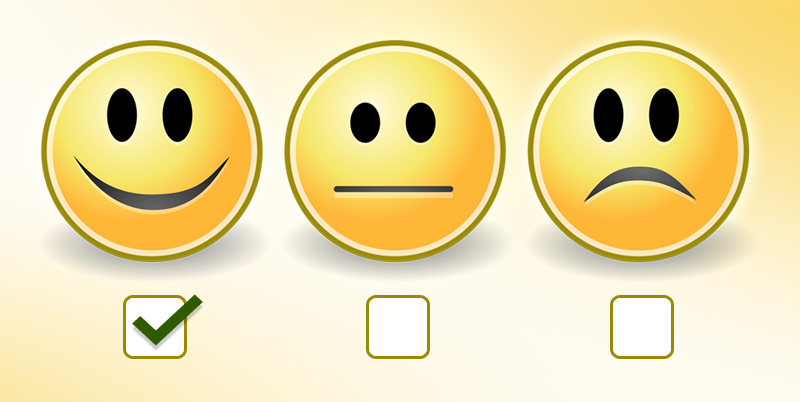
\includegraphics[width=\linewidth,keepaspectratio]{sent}
\end{center}
\end{frame}


%%%%%%%%%%%%%%%%%%%%%%%%%%%%%%%%%%%%%%%%%%%%%%%%%%%%%%%%%%%
\begin{frame}[fragile]\frametitle{Sentiment Analysis}
Restaurant/hotel recommendation, Product reviews
\begin{center}
\includegraphics[width=\linewidth,keepaspectratio]{recco}
\end{center}
\end{frame}

%%%%%%%%%%%%%%%%%%%%%%%%%%%%%%%%%%%%%%%%%%%%%%%%%%%%%%%%%%%
\begin{frame}[fragile]\frametitle{Sentiment Analysis}
Text analytics in financial services

\begin{center}
\includegraphics[width=\linewidth,keepaspectratio]{finnlp}
\end{center}
\end{frame}


%%%%%%%%%%%%%%%%%%%%%%%%%%%%%%%%%%%%%%%%%%%%%%%%%%%%%%%%%%%
\begin{frame}[fragile]\frametitle{NLP in today's time}
Trends:
	\begin{itemize}
	\item An enormous amount of information is now available in machine readable form as natural language text (newspapers, web pages, medical records, financial filings, product reviews, discussion forums, etc.)
	\item Conversational agents are becoming an important form of human-computer communication
	\item Much of human-human interaction is now mediated by computers via social media
	\end{itemize}
Collectively, this means that copious data is available to be used in the development of NLP systems.

\end{frame}
%%%%%%%%%%%%%%%%%%%%%%%%%%%%%%%%%%%%%%%%%%%%%%%%%%%%%%%%%%%
\begin{frame}[fragile]\frametitle{Level of difficulties}

	\begin{itemize}
	\item Easy (mostly solved)
		\begin{itemize}
		\item Spell and grammar checking
		\item Some text categorization tasks
		\item Some named-entity recognition tasks
		\end{itemize}
	\item Intermediate (good progress)
		\begin{itemize}
		\item Information retrieval
		\item Sentiment analysis
		\item Machine translation
		\item Information extraction
		\end{itemize}	
	\item Difficult (still hard)
		\begin{itemize}
		\item Question answering
		\item Summarization
		\item Dialog systems
		\end{itemize}	
	\end{itemize}

\end{frame}


%%%%%%%%%%%%%%%%%%%%%%%%%%%%%%%%%%%%%%%%%%%%%%%%%%%%%%%%%%%%
%\begin{frame}[fragile]\frametitle{How?}
%\begin{itemize}
%\item All of these applications operate by exploiting underlying regularities underlying all human languages.
%\item Sometimes in complex ways, sometimes in pretty trivial ways.
%\end{itemize}
%\begin{center}
%\includegraphics[width=\linewidth,keepaspectratio]{nlppipe}
%\end{center}
%\end{frame}

%%%%%%%%%%%%%%%%%%%%%%%%%%%%%%%%%%%%%%%%%%%%%%%%%%%%%%%%%%%
\begin{frame}
  \begin{center}
    {\Large Langauge Representation: How to make text computable?}
  \end{center}
\end{frame}


%%%%%%%%%%%%%%%%%%%%%%%%%%%%%%%%%%%%%%%%%%%%%%%%%%%%%%%%%%%
\begin{frame}[fragile]\frametitle{Document Representation \& Language Model}
\begin{itemize}
\item How to represent a document?
\item Make it computable
\item How to infer the relationship among documents or identify the structure within a document?
\item Knowledge discovery
\item Language Model and N-Grams

\end{itemize}
\end{frame}

% %%%%%%%%%%%%%%%%%%%%%%%%%%%%%%%%%%%%%%%%%%%%%%%%%%%%%%%%%%%
% \begin{frame}[fragile]\frametitle{How to represent a document?}
% \begin{itemize}
% \item Represent by a string? No semantic meaning
% \item Represent by a list of sentences? Sentence is just like a short document (recursive definition)
% \end{itemize}
% \begin{center}
% \includegraphics[width=0.6\linewidth,keepaspectratio]{nlpstr}
% \end{center}
% \end{frame}

%%%%%%%%%%%%%%%%%%%%%%%%%%%%%%%%%%%%%%%%%%%%%%%%%%%%%%%%%%%
\begin{frame}[fragile]\frametitle{Bag-of-Words representation}
Term as the basis for vector space
\begin{itemize}
\item Doc1: Text mining is to identify useful information.
\item Doc2: Useful information is mined from text.
\item Doc3: Apple is delicious.
\end{itemize}
\begin{center}
\includegraphics[width=\linewidth,keepaspectratio]{bowtable}
\end{center}
\end{frame}


%%%%%%%%%%%%%%%%%%%%%%%%%%%%%%%%%%%%%%%%%%%%%%%%%%%%%%%%%%%%%%%%%%%%%%%%%%%%%%%%%%
\begin{frame}[fragile]\frametitle{What are Word Vectors/Embeddings?}
\begin{itemize}
\item Word Embeddings are the texts converted into numbers
\item There may be different numerical representations of  same text. 
\item Many Machine Learning algorithms and almost all Deep Learning Architectures are incapable of processing strings or plain text in their raw form. 
\item They require numbers as inputs to perform any sort of job, be it classification, regression etc. in broad terms.
\item So, for the computer to be able to ''understand'' a vector representation of a word is required.
\end{itemize}
\end{frame}

%%%%%%%%%%%%%%%%%%%%%%%%%%%%%%%%%%%%%%%%%%%%%%%%%%%%%%%%%%%%%%%%%%%%%%%%%%%%%%%%%%
\begin{frame}[fragile]\frametitle{Different types of Word Vectors}
\begin{itemize}
\item (Traditional) Frequency based Embedding:
\begin{itemize}
\item One-hot
\item Count Vector
\item TF-IDF Vector
\item Co-Occurrence Vector
\end{itemize}
\item (Modern) Prediction based Embedding:
\begin{itemize}
\item Word2vec  (Google)
\item Global Vector Representations (GloVe)   (Stanford)
\end{itemize}
\end{itemize}
\end{frame}



%%%%%%%%%%%%%%%%%%%%%%%%%%%%%%%%%%%%%%%%%%%%%%%%%%%%%%%%%%%%%%%%%%%%%%%%%%%%%%%%%%
\begin{frame}[fragile]\frametitle{One Hot}
One-hot:  Suppose our vocabulary has only five words: King, Queen, Man, Woman, and Child. We could encode the word `Queen' as:
\begin{center}
\includegraphics[width=0.8\linewidth,keepaspectratio]{word40}
\end{center}
No meaningful comparison possible.
\end{frame}




% %%%%%%%%%%%%%%%%%%%%%%%%%%%%%%%%%%%%%%%%%%%%%%%%%%%%%%%%%%%%%%%%%%%%%%%%%%%%%%%%%%
% \begin{frame}[fragile]\frametitle{Count Vector}
% \begin{itemize}
% \item Corpus:
% \begin{itemize}
% \item D1: He is a lazy boy. She is also lazy.
% \item D2: Neeraj is a lazy person.
% \end{itemize}
% \item Dictionary is a list of unique tokens(words) =['He','She','lazy','boy','Neeraj','person'] 
% \item Count Matrix:
% \begin{center}
% \includegraphics[width=\linewidth,keepaspectratio]{word29}
% \end{center}
% \end{itemize}
% \end{frame}

% %%%%%%%%%%%%%%%%%%%%%%%%%%%%%%%%%%%%%%%%%%%%%%%%%%%%%%%%%%%%%%%%%%%%%%%%%%%%%%%%%%
% \begin{frame}[fragile]\frametitle{Count Vector}
% \begin{center}
% \includegraphics[width=0.8\linewidth,keepaspectratio]{word30}
% \end{center}
% \end{frame}

% %%%%%%%%%%%%%%%%%%%%%%%%%%%%%%%%%%%%%%%%%%%%%%%%%%%%%%%%%%%%%%%%%%%%%%%%%%%%%%%%%%
% \begin{frame}[fragile]\frametitle{TF-IDF vectorization}
% \begin{itemize}
% \item It takes into account not just the occurrence of a word in a single document but in the entire corpus.
% \item Down weight the common words occurring in almost all documents and give more importance to words that appear in a subset of documents.
% \item Corpus:
% \begin{center}
% \includegraphics[width=0.8\linewidth,keepaspectratio]{word31}
% \end{center}
% \end{itemize}
% \end{frame}

% %%%%%%%%%%%%%%%%%%%%%%%%%%%%%%%%%%%%%%%%%%%%%%%%%%%%%%%%%%%%%%%%%%%%%%%%%%%%%%%%%%
% \begin{frame}[fragile]\frametitle{TF-IDF vectorization}
% \begin{itemize}
% \item TF = (Number of times term t appears in a document)/(Number of terms in the document)
% \item So, TF(This,Document1) = 1/8  and TF(This, Document2)=1/5
% \item IDF = log(N/n), where, N is the number of documents and n is the number of documents a term t has appeared in.
% \item So, IDF(This) = log(2/2) = 0.
% \item TFIDF = TF*IDF
% \item Dictionary is made of a list of unique tokens(words) 
% \item Similar to Count Matrix, TFIDF matrix is made with TFIDF values in it.
% \end{itemize}
% \end{frame}


% %%%%%%%%%%%%%%%%%%%%%%%%%%%%%%%%%%%%%%%%%%%%%%%%%%%%%%%%%%%%%%%%%%%%%%%%%%%%%%%%%%
% \begin{frame}[fragile]\frametitle{Co-Occurrence Matrix}
% \begin{itemize}
% \item Co-occurrence ' For a given corpus, the co-occurrence of a pair of words say w1 and w2 is the number of times they have appeared together in a Context Window.
% \item Context Window ' Context window is specified by a number and the direction. So what does a context window of 2 (around) means?
% \begin{center}
% \includegraphics[width=0.6\linewidth,keepaspectratio]{word32}
% \end{center}
% \item For Corpus ='' He is not lazy. He is intelligent. He is smart.''
% \end{itemize}
% \begin{center}
% \includegraphics[width=0.5\linewidth,keepaspectratio]{word33}
% \end{center}
% \end{frame}

% %%%%%%%%%%%%%%%%%%%%%%%%%%%%%%%%%%%%%%%%%%%%%%%%%%%%%%%%%%%%%%%%%%%%%%%%%%%%%%%%%%
% \begin{frame}[fragile]\frametitle{Co-Occurrence Matrix}
% Red box- It is the number of times 'He' and 'is' have appeared in the context window 2 and it can be seen that the count turns out to be 4. 
% \begin{center}
% \includegraphics[width=0.5\linewidth,keepaspectratio]{word34}
% \end{center}
% While the word 'lazy' has never appeared with'intelligent' in the context window and therefore has been assigned 0 in the blue box.
% \end{frame}



%%%%%%%%%%%%%%%%%%%%%%%%%%%%%%%%%%%%%%%%%%%%%%%%%%%%%%%%%%%%%%%%%%%%%%%%%%%%%%%%%%
\begin{frame}[fragile]\frametitle{Good Vector Representation}
\begin{itemize}
\item To have ''Semantic'' (meaning-wise) representation, the Similar words should be close to each other in the hyper dimensional space.
\item Non-similar words should be far apart from each other in the hyper dimensional space.
\end{itemize}
\end{frame}

%%%%%%%%%%%%%%%%%%%%%%%%%%%%%%%%%%%%%%%%%%%%%%%%%%%%%%%%%%%%%%%%%%%%%%%%%%%%%%%%%%
\begin{frame}[fragile]\frametitle{Good Vector Representation}
\begin{itemize}
\item Traditional One Hot Encoding:
	\begin{itemize}
	\item Apple = [1, 0, 0]
	\item Orange = [0, 1, 0]
	\item Plane = [0, 0, 1]
	\end{itemize}
\begin{center}
\includegraphics[width=0.6\linewidth,keepaspectratio]{word23_1}
\end{center}
\item Very few cells participate in the representation.
\end{itemize}
\end{frame}



%%%%%%%%%%%%%%%%%%%%%%%%%%%%%%%%%%%%%%%%%%%%%%%%%%%%%%%%%%%%%%%%%%%%%%%%%%%%%%%%%%
\begin{frame}[fragile]\frametitle{Word2Vec}
Word2vec  (Google): a distributed representation of a word is used and not sparse like One-Hot.
\begin{center}
\includegraphics[width=0.8\linewidth,keepaspectratio]{word41}
\end{center}
Represent in some abstract way the `meaning' of a word.

\end{frame}

%%%%%%%%%%%%%%%%%%%%%%%%%%%%%%%%%%%%%%%%%%%%%%%%%%%%%%%%%%%%%%%%%%%%%%%%%%%%%%%%%%
\begin{frame}[fragile]\frametitle{Word Distributed Representation - Word2Vec}
\begin{itemize}
\item All vector cells participate in representing each word.
\item Words are represented by real valued dense vectors of significantly smaller dimensions (e.g. 100 - 1000).
\item  Intuition: consider each vector cell as a representative of some feature.
\begin{center}
\includegraphics[width=\linewidth,keepaspectratio]{word24}
\end{center}
\end{itemize}
\end{frame}




%%%%%%%%%%%%%%%%%%%%%%%%%%%%%%%%%%%%%%%%%%%%%%%%%%%%%%%%%%%%%%%%%%%%%%%%%%%%%%%%%%
\begin{frame}[fragile]\frametitle{Word Representations Comparison}

\adjustbox{valign=t}{
\begin{minipage}{0.45\linewidth}
Traditional Method  - Bag of Words Model

\begin{itemize}
\item Uses one hot encoding
\item Each word in the vocabulary is represented by one bit position in a HUGE vector.
\item For example, with a vocabulary of 10000 words, and ''Hello'' is the 4th word in the dictionary:  \lstinline|0 0 0 1 0 0  . . . . . . . 0 0 0 0 |
\item Context information is not utilized
\end{itemize}
\end{minipage}
}
\hfill
\adjustbox{valign=t}{
\begin{minipage}{0.45\linewidth}
Modern - Word Vectors

\begin{itemize}
\item Stores each word in as a point in space, represented by a vector of fixed number of dimensions (generally 300)
\item Unsupervised, built just by reading huge corpus
\item For example, ''Hello'' might be represented as :  \lstinline| [0.4, -0.11, 0.55, 0.3 . . . 0.1, 0.02]|
\item Context information is utilized
\end{itemize}
\end{minipage}
}
\end{frame}






%%%%%%%%%%%%%%%%%%%%%%%%%%%%%%%%%%%%%%%%%%%%%%%%%%%%%%%%%%%%%%%%%%%%%%%%%%%%%%%%%%
\begin{frame}[fragile]\frametitle{Examples}
Vectors for King, Man, Queen, \& Woman:
\begin{center}
\includegraphics[width=0.5\linewidth,keepaspectratio]{word42}
\end{center}


\begin{center}
\includegraphics[width=0.5\linewidth,keepaspectratio]{word44}
\end{center}

\end{frame}

%%%%%%%%%%%%%%%%%%%%%%%%%%%%%%%%%%%%%%%%%%%%%%%%%%%%%%%%%%%%%%%%%%%%%%%%%%%%%%%%%%
\begin{frame}[fragile]\frametitle{Examples}
Gender relation:
\begin{center}
\includegraphics[width=0.4\linewidth,keepaspectratio]{word45}
\end{center}
Plural relation:

\begin{center}
\includegraphics[width=0.4\linewidth,keepaspectratio]{word46}
\end{center}

\end{frame}

%%%%%%%%%%%%%%%%%%%%%%%%%%%%%%%%%%%%%%%%%%%%%%%%%%%%%%%%%%%%%%%%%%%%%%%%%%%%%%%%%%
\begin{frame}[fragile]\frametitle{Examples}
Word pair relationships:
\begin{center}
\includegraphics[width=0.8\linewidth,keepaspectratio]{word47}
\end{center}
\end{frame}

%%%%%%%%%%%%%%%%%%%%%%%%%%%%%%%%%%%%%%%%%%%%%%%%%%%%%%%%%%%%%%%%%%%%%%%%%%%%%%%%%%
\begin{frame}[fragile]\frametitle{Examples}
Country-capital city relationship:

\begin{center}
\includegraphics[width=0.8\linewidth,keepaspectratio]{word48}
\end{center}

\end{frame}

%%%%%%%%%%%%%%%%%%%%%%%%%%%%%%%%%%%%%%%%%%%%%%%%%%%%%%%%%%%%%%%%%%%%%%%%%%%%%%%%%%
\begin{frame}[fragile]\frametitle{The Power of Word2Vecs}

\begin{itemize}
\item They provide a fresh perspective to ALL  problems in NLP, and not just solve one problem.
\item Technological Improvement
\item Rise of deep learning since 2006 (Big Data + GPUs  + Work done by Andrew Ng, Yoshua Bengio, Yann Lecun and Geoff Hinton)
\item Application of Deep Learning to NLP - led by Yoshua Bengio,  Christopher Manning, Richard Socher, Tomas Mikalov
\item The need for unsupervised learning . (Supervised learning tends to be excessively dependent on hand-labeled data and often does not scale)
\end{itemize}
\end{frame}

% %%%%%%%%%%%%%%%%%%%%%%%%%%%%%%%%%%%%%%%%%%%%%%%%%%%%%%%%%%%
% \begin{frame}[fragile]\frametitle{Vector space model}
% \begin{itemize}
% \item Represent documents by concept vectors
% \begin{itemize}
% \item Each concept defines one dimension
% \item $k$ concepts define a high-dimensional space
% \item Element of vector corresponds to concept weight
% E.g.,$d=(x_1,\ldots,x_k)$, $x_i$ is ``importance'' of concept $i$ in $d$
% \end{itemize}
% \item Distance between the vectors in this concept space: Relationship among documents  	
% \end{itemize}
% \end{frame}

% %%%%%%%%%%%%%%%%%%%%%%%%%%%%%%%%%%%%%%%%%%%%%%%%%%%%%%%%%%%
% \begin{frame}[fragile]\frametitle{Vector space model Example}
% All documents are projected into this concept space
% \begin{center}
% \includegraphics[width=0.8\linewidth,keepaspectratio]{vsapp}
% \end{center}
% \end{frame}



% %%%%%%%%%%%%%%%%%%%%%%%%%%%%%%%%%%%%%%%%%%%%%%%%%%%%%%%%%%%
% \begin{frame}[fragile]\frametitle{(Old) Linguistics Terminology}
% Phonetics and phonology: The study of  linguistic sounds and their relations to words
% \begin{center}
% \includegraphics[width=0.6\linewidth,keepaspectratio]{phono}
% \end{center}
% \end{frame}


% %%%%%%%%%%%%%%%%%%%%%%%%%%%%%%%%%%%%%%%%%%%%%%%%%%%%%%%%%%%
% \begin{frame}[fragile]\frametitle{(Old) Linguistics Terminology}
% \begin{itemize}
% \item Morphology: The study of internal structures of words and how they can be modified.
% \item Parsing complex words into their components.
% \item The study of the forms of things, words in particular.
% \item Consider pluralization for English:
% \item Orthographic Rules: puppy to  puppies
% \item Morphological Rules: goose to geese or fish
% \end{itemize}
% \end{frame}

% %%%%%%%%%%%%%%%%%%%%%%%%%%%%%%%%%%%%%%%%%%%%%%%%%%%%%%%%%%%
% \begin{frame}[fragile]\frametitle{(Old) Linguistics Terminology}
% Semantics: The study of the meaning of words, and how these combine to  form the meanings of sentences
% \begin{itemize}
% \item Synonymy: fall \& autumn
% \item Hypernymy \& hyponymy (is a): animal \& dog
% \item Meronymy (part of): finger \& hand 
% \item Homonymy: fall (verb \& season)
% \item Antonymy: big \& small
% \end{itemize}
% \end{frame}
%
%%%%%%%%%%%%%%%%%%%%%%%%%%%%%%%%%%%%%%%%%%%%%%%%%%%%%%%%%%%%
%\begin{frame}[fragile]\frametitle{NLP Terminology}
%Pragmatics: The study of the meaning of words, and how these combine to  form the meanings of sentences
%\begin{itemize}
%\item Social use of language
%\item The study of how language is used to accomplish goals, and the influence of context on meaning
%\item  Understanding the aspects of a language which depends on situation and world knowledge
%\end{itemize}
%Give me the salt! \\
%Could you please give me the salt?
%\end{frame}


%%%%%%%%%%%%%%%%%%%%%%%%%%%%%%%%%%%%%%%%%%%%%%%%%%%%%%%%%%%%
%\begin{frame}[fragile]\frametitle{NLP Terminology}
%Discourse: The study of linguistic units larger than a single statement.\\
%John reads a book. {\bf He} borrowed {\bf it} from {\bf his} friend.
%\begin{center}
%\includegraphics[width=\linewidth,keepaspectratio]{dis}
%\end{center}
%\end{frame}

%%%%%%%%%%%%%%%%%%%%%%%%%%%%%%%%%%%%%%%%%%%%%%%%%%%%%%%%%%%
\begin{frame}
  \begin{center}
    {\Large NLP Activities: How to process text?}
  \end{center}
\end{frame}


%%%%%%%%%%%%%%%%%%%%%%%%%%%%%%%%%%%%%%%%%%%%%%%%%%%%%%%%%%%
\begin{frame}[fragile]\frametitle{Document/Section splitting}
Document/Section splitting: Splitting a text into sections
\begin{center}
\includegraphics[width=\linewidth,keepaspectratio]{secsplit}
\end{center}
\end{frame}


%%%%%%%%%%%%%%%%%%%%%%%%%%%%%%%%%%%%%%%%%%%%%%%%%%%%%%%%%%%
\begin{frame}[fragile]\frametitle{Sentence splitting}
Sentence splitting: Splitting a text into sentences
\begin{center}
\includegraphics[width=\linewidth,keepaspectratio]{setsplit}
\end{center}
\end{frame}

%%%%%%%%%%%%%%%%%%%%%%%%%%%%%%%%%%%%%%%%%%%%%%%%%%%%%%%%%%%
\begin{frame}[fragile]\frametitle{Tokenization}
Tokenization
		\begin{itemize}
		\item  Process of breaking a stream of text up into tokens ( = words, phrases, symbols, or other meaningful elements)
		\item  Typically performed at the ``word'' level
		\item  Not easy: Hewlett-Packard, U.S.A., in some languages there is no ``space'' between words!
		\end{itemize}
\end{frame}

%%%%%%%%%%%%%%%%%%%%%%%%%%%%%%%%%%%%%%%%%%%%%%%%%%%%%%%%%%%
\begin{frame}[fragile]\frametitle{Stemming}
Stemming
		\begin{itemize}
		\item  Reduces similar words to a given ``stem''
    \item E.g. detects, detected, detecting, detect : detect (stem).
    \item Usually set of rules for suffix stripping 
    \item Most popular for English: Porter's Algorithm 
    \item 36\% reduction in indexing vocabulary (English)
    \item Linguistic correctness of resulting stems not necessary (sensitivities : sensit)
		\end{itemize}
\end{frame}

%%%%%%%%%%%%%%%%%%%%%%%%%%%%%%%%%%%%%%%%%%%%%%%%%%%%%%%%%%%
\begin{frame}[fragile]\frametitle{Lemmatization}
Lemmatization
		\begin{itemize}
		\item  Uses a vocabulary and full morphological analysis of words
    \item Aims to remove inflectional endings only 
    \item Return the base or dictionary form of a word, which is known as the lemma.
    \item E.g. saw :  see,      \\              been, was : be
		\end{itemize}
\end{frame}

%%%%%%%%%%%%%%%%%%%%%%%%%%%%%%%%%%%%%%%%%%%%%%%%%%%%%%%%%%%
\begin{frame}[fragile]\frametitle{Part-of-speech tagging}
Part-of-speech tagging: Assigning a syntatic tag to each word in a sentence
\begin{center}
\includegraphics[width=\linewidth,keepaspectratio]{postag}
\end{center}
\end{frame}

%%%%%%%%%%%%%%%%%%%%%%%%%%%%%%%%%%%%%%%%%%%%%%%%%%%%%%%%%%%
\begin{frame}[fragile]\frametitle{Parsing}
Parsing: Building the syntactic tree of a sentence
\begin{center}
\includegraphics[width=\linewidth,keepaspectratio]{parse}
\end{center}
\end{frame}

%%%%%%%%%%%%%%%%%%%%%%%%%%%%%%%%%%%%%%%%%%%%%%%%%%%%%%%%%%%
\begin{frame}[fragile]\frametitle{Parsing}
$ ((DaimlerChryslers shares)_{NP} (rose (three eights)_{ NUMP} (to 22)_{PP-NUM}  )_{VP}  )_{S}$
\begin{center}
\includegraphics[width=0.8\linewidth,keepaspectratio]{tree}
\end{center}
\end{frame}


%%%%%%%%%%%%%%%%%%%%%%%%%%%%%%%%%%%%%%%%%%%%%%%%%%%%%%%%%%%
\begin{frame}[fragile]\frametitle{Syntax Tree}
Syntax: Sample English grammar
\begin{center}
\includegraphics[width=\linewidth,keepaspectratio]{grammar}
\end{center}
\end{frame}

%%%%%%%%%%%%%%%%%%%%%%%%%%%%%%%%%%%%%%%%%%%%%%%%%%%%%%%%%%%
\begin{frame}[fragile]\frametitle{Named-entity recognition}
Named-entity recognition: Identifying pre-defined entity types in a sentence
\begin{center}
\includegraphics[width=\linewidth,keepaspectratio]{ner}
\end{center}
\end{frame}

%%%%%%%%%%%%%%%%%%%%%%%%%%%%%%%%%%%%%%%%%%%%%%%%%%%%%%%%%%%
\begin{frame}[fragile]\frametitle{Topic modelings}
Topic modeling: Identifying structures in the text corpus

\begin{center}
\includegraphics[width=\linewidth,keepaspectratio]{topic}
\end{center}
\end{frame}


%%%%%%%%%%%%%%%%%%%%%%%%%%%%%%%%%%%%%%%%%%%%%%%%%%%%%%%%%%%%
%\begin{frame}[fragile]\frametitle{NLP Activities}
%Semantics
%		\begin{itemize}
%	\item How can computers use/understand human knowledge?
%    \item Either use human-made knowledge bases (called ontologies)
%    		\begin{itemize}
%    \item WordNet 
%    \item FrameNet
%    \item Etc.
%    		\end{itemize}
%    \item Try to build knowledge bases on their own by analyzing large collections of texts (maybe use some human ``seeds'' for relations and concepts)
%    		\begin{itemize}
%    \item NELL (Never Ending Language Learning)
%    \item Probase
%    \item Freebase, Dbpedia
%    \item Google Knowledge Graph
%    		\end{itemize}
%    \item Try to assess meaning from the context of words
%    		\begin{itemize}
%    \item The meaning of a word is actually distributed in the ``meaning'' of the words used together with it
%    \item Compute these distributed word embedding
%    		\end{itemize}
%		\end{itemize}
%\end{frame}


%%%%%%%%%%%%%%%%%%%%%%%%%%%%%%%%%%%%%%%%%%%%%%%%%%%%%%%%%%%%
%\begin{frame}[fragile]\frametitle{NLP Activities}
%Word sense disambiguation : Figuring out the exact meaning of a word or entity
%\begin{center}
%\includegraphics[width=\linewidth,keepaspectratio]{wordsense}
%\end{center}
%\end{frame}

%%%%%%%%%%%%%%%%%%%%%%%%%%%%%%%%%%%%%%%%%%%%%%%%%%%%%%%%%%%%
%\begin{frame}[fragile]\frametitle{NLP Activities}
%Semantic role labeling :  Extracting subject-predicate-object triples from a sentence
%\begin{center}
%\includegraphics[width=\linewidth,keepaspectratio]{rolelab}
%\end{center}
%\end{frame}


%%%%%%%%%%%%%%%%%%%%%%%%%%%%%%%%%%%%%%%%%%%%%%%%%%%%%%%%%%%
\begin{frame}[fragile]\frametitle{Word embeddings}
Word embeddings: Compute a vector representing the distributed representation for every word
\begin{center}
\includegraphics[width=\linewidth,keepaspectratio]{wordvec}
\end{center}
\end{frame}




